\chapter{Connect Firebase To App}
\section{Create Firebase Project}
\subitem{
	Open Browser and go to "https://console.firebase.google.com" to create app in firebase console to add to your app in android studio
	\begin{figure}[H]
		\centering
		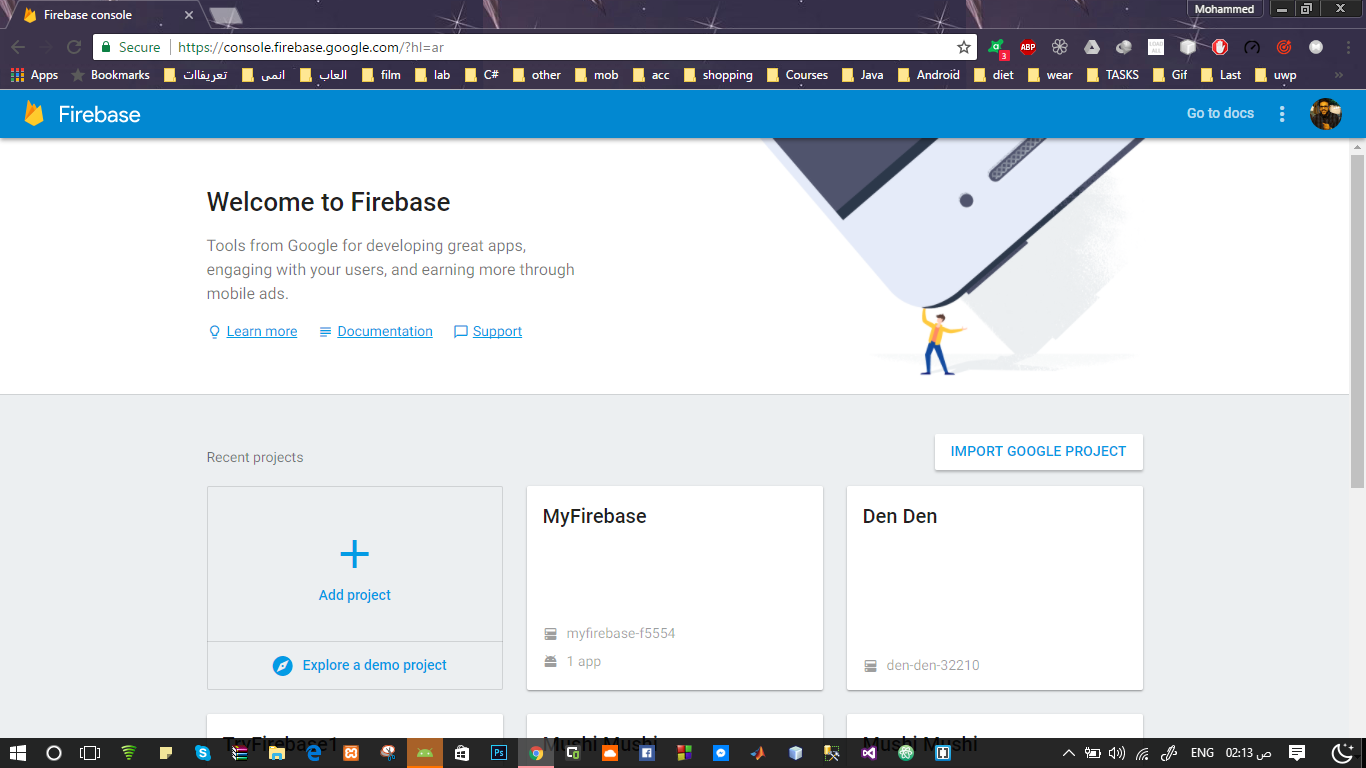
\includegraphics[height=3in]{./TeX_files/pic2}
		\caption[optional caption]{Firebase Console}
		\label{Fig:Tobias}
	\end{figure}
	
	click on Add Project to display this form and enter the name of your app and your Country/region
	\begin{figure}[H]
		\centering
		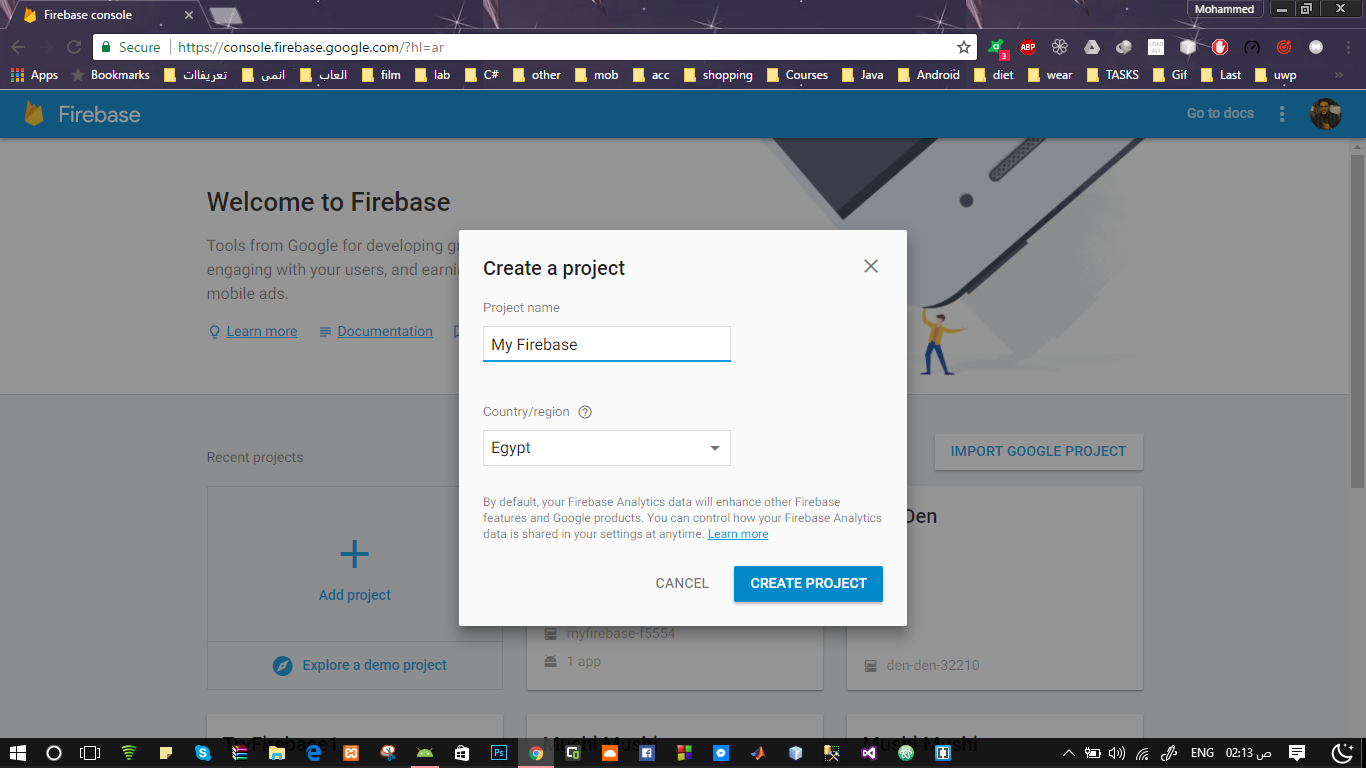
\includegraphics[height=3in]{./TeX_files/pic3}
		\caption[optional caption]{Create new project}
		\label{Fig:Tobias}
	\end{figure}
	After enter the data and click on 'Create Project'
	 \begin{figure}[H]
	 	\centering
	 	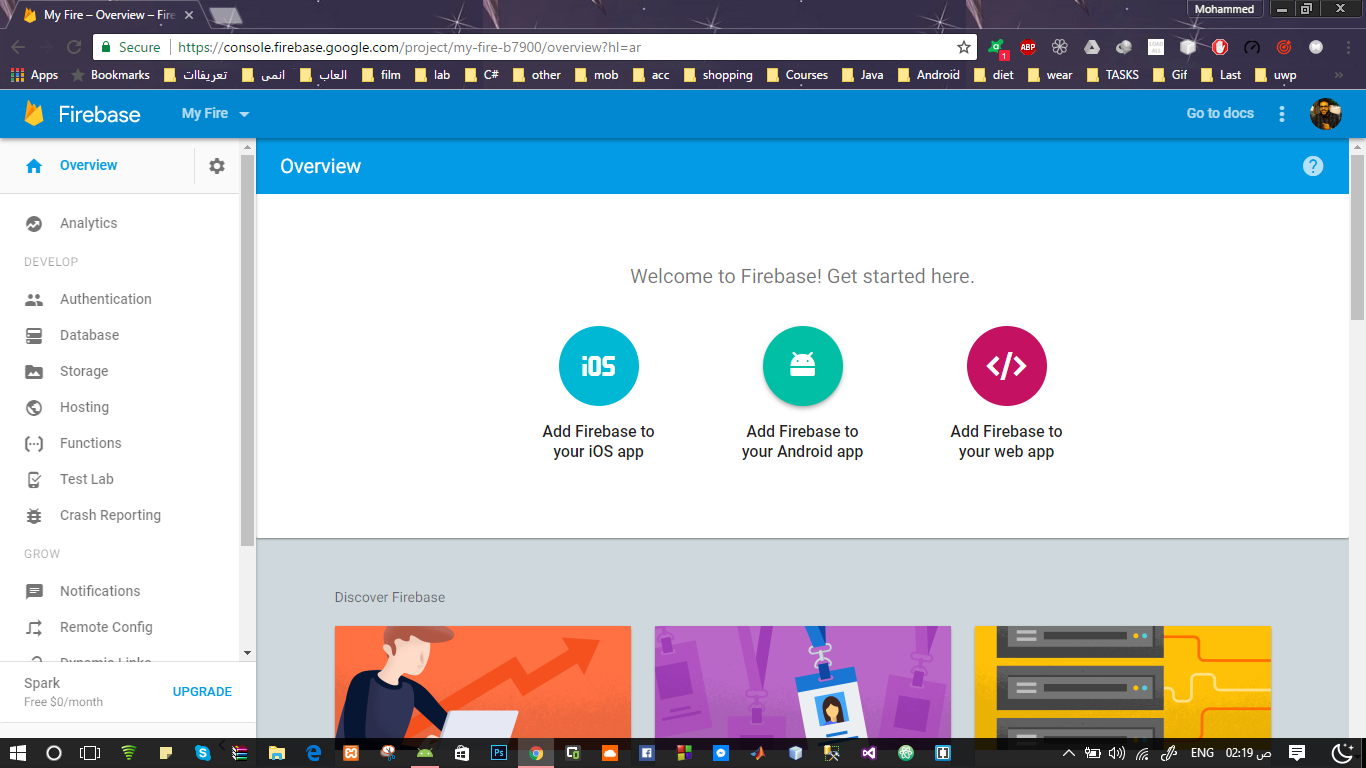
\includegraphics[height=3in]{./TeX_files/pic4}
	 	\caption[optional caption]{Choose Your platform}
	 	\label{Fig:Tobias}
	 \end{figure}
	choose platform which i need to built my app in , in our case we choose 'Android' as platform
	\begin{figure}[H]
		\centering
		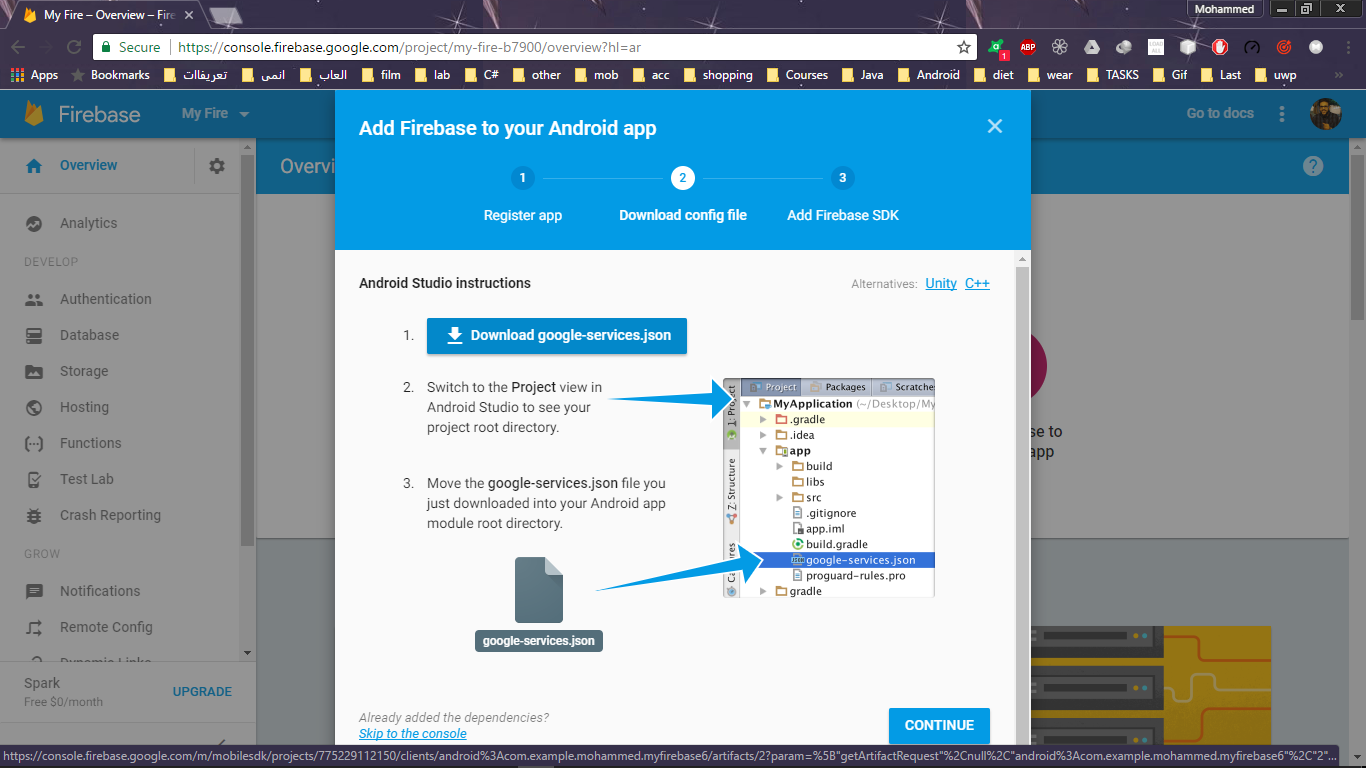
\includegraphics[height=3in]{./TeX_files/pic5}
		\caption[optional caption]{Download your json file}
		\label{Fig:Tobias}
	\end{figure}
	}
\section{Add Firebase To App}
\subitem{
	Open Your Android studio add your Json file which your downloaded on your app file 
	\begin{figure}[H]
		\centering
		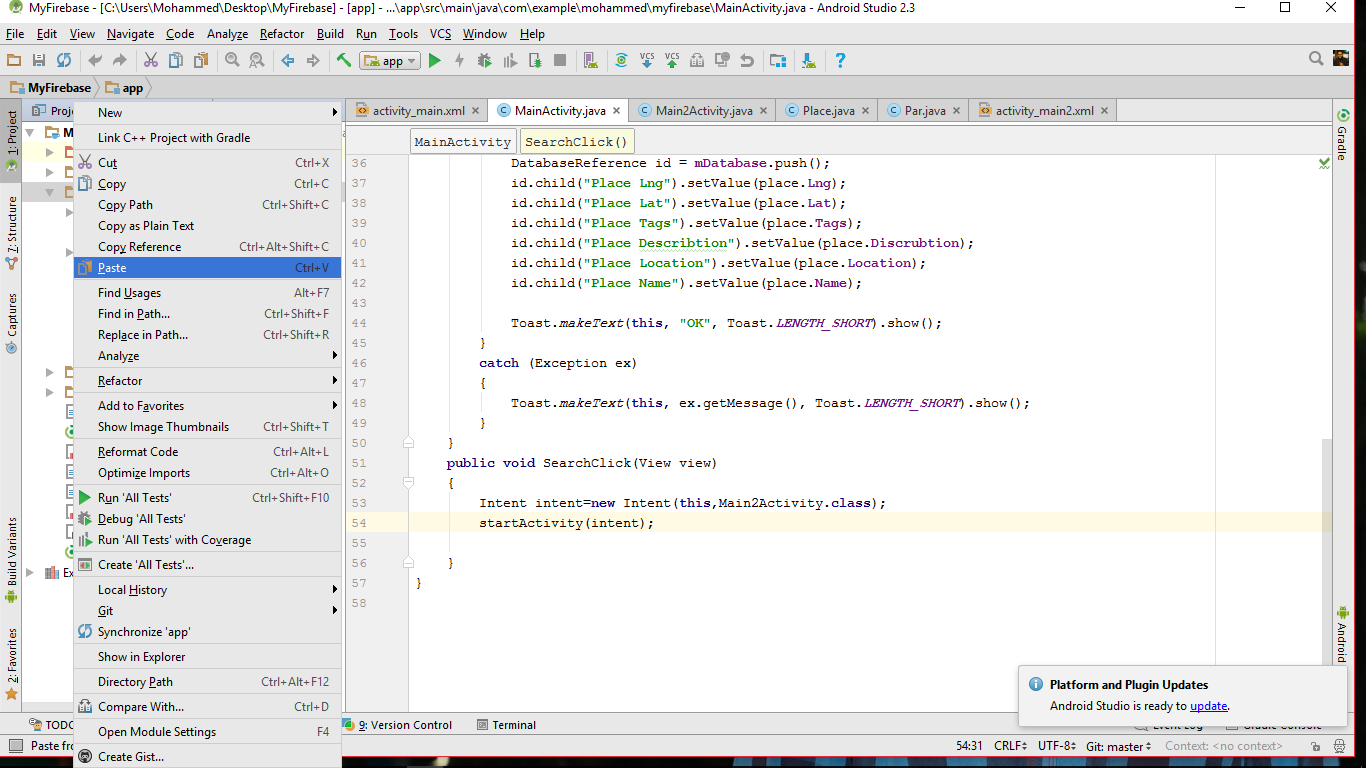
\includegraphics[height=3in]{./TeX_files/pic6}
		\caption[optional caption]{Add json file to your app}
		\label{Fig:Tobias}
	\end{figure}
	\begin{figure}[H]
		\centering
		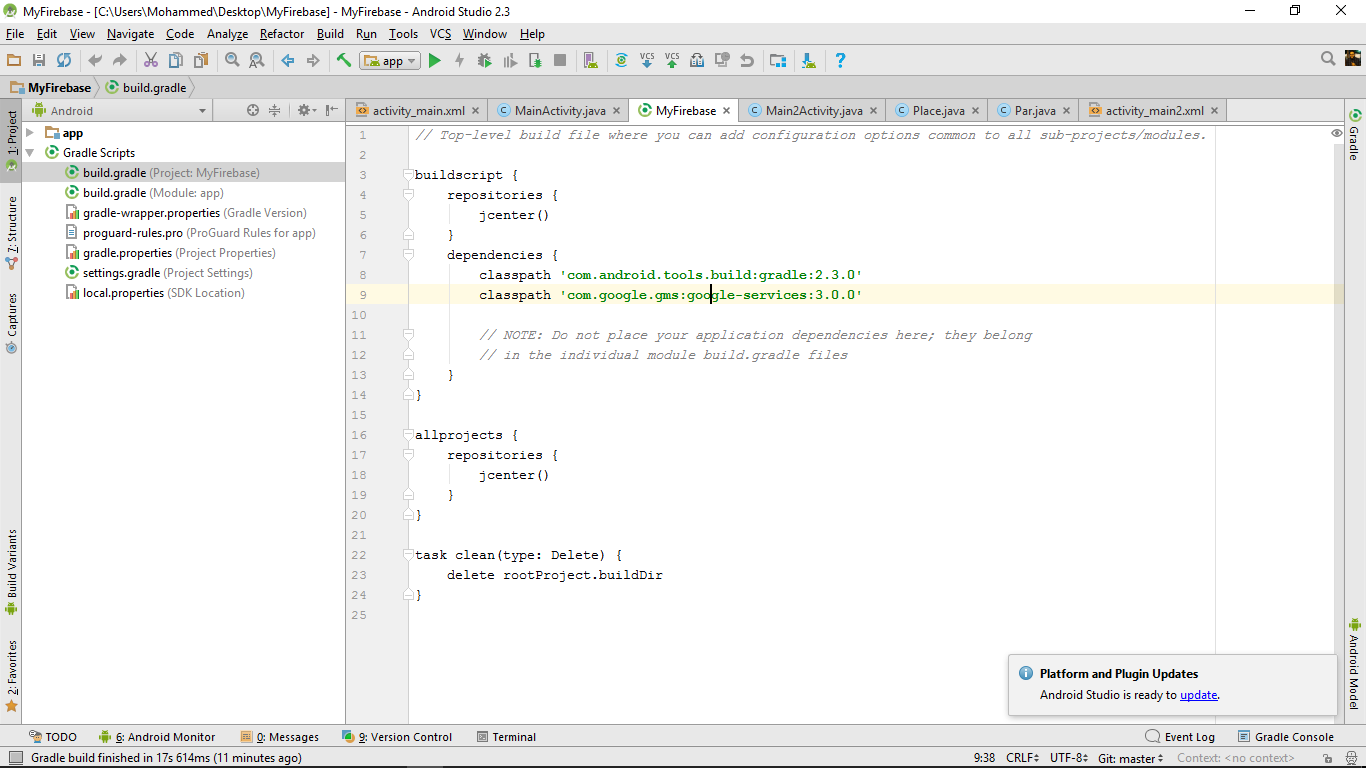
\includegraphics[height=3in]{./TeX_files/pic7}
		\caption[optional caption]{Add classpath to Gridle Project }
		\label{Fig:Tobias}
	\end{figure}
	\begin{figure}[H]
		\centering
		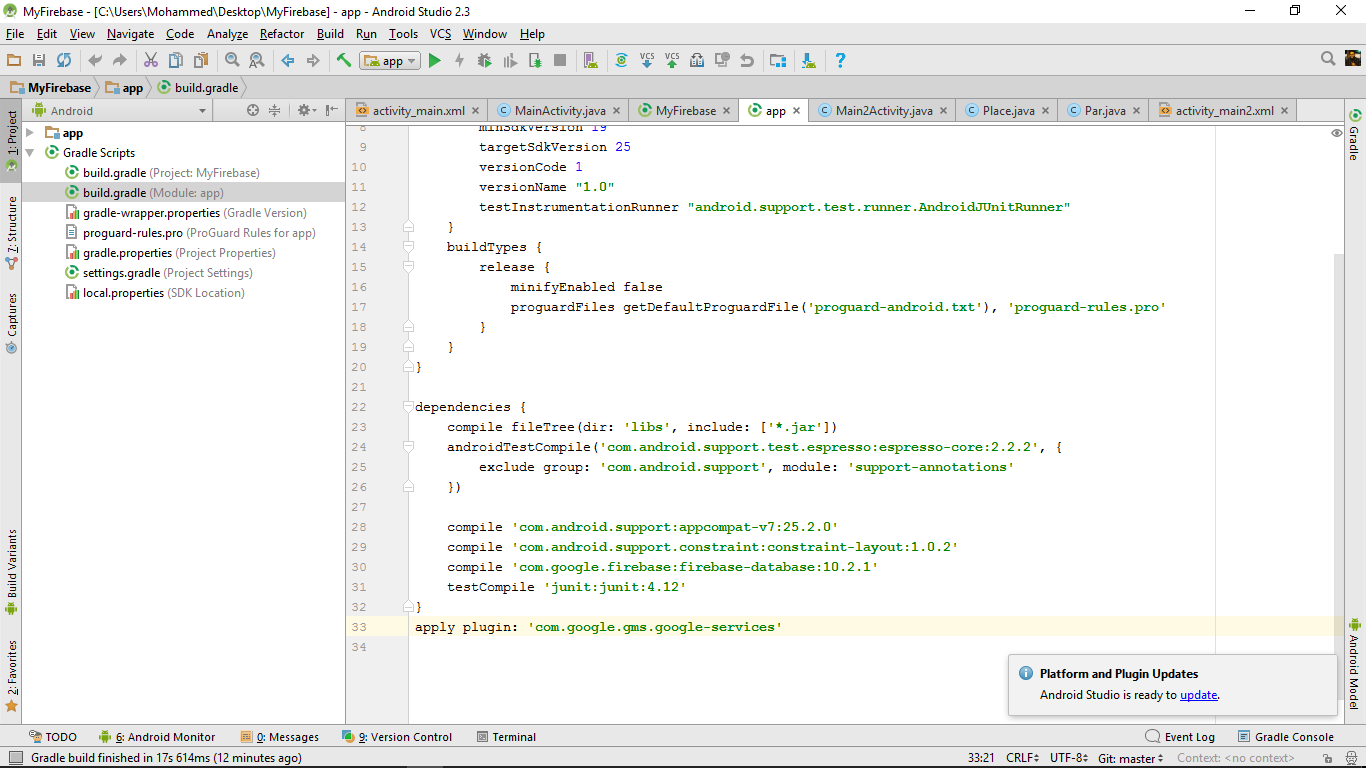
\includegraphics[height=3in]{./TeX_files/pic8}
		\caption[optional caption]{Add Compile in Gridle App}
		\label{Fig:Tobias}
	\end{figure}
	
	your app in android studio connected with your firebase
   app in firebase console
	}
\section{Add Network Permission}
\subitem{
	Go to manifest file and add the permission to access the internet
	
	\begin{figure}[H]
		\centering
		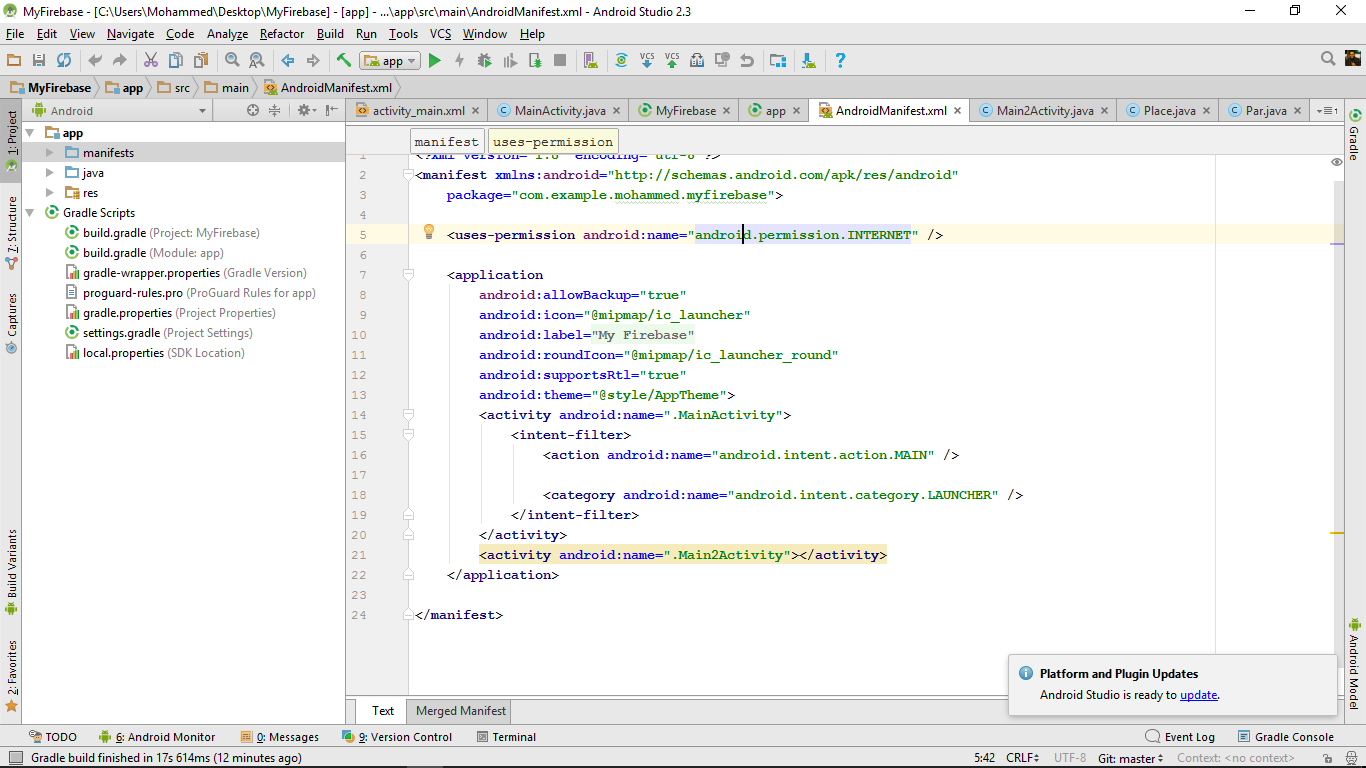
\includegraphics[height=3in]{./TeX_files/pic9}
		\caption[optional caption]{Add Compile in Gridle App}
		\label{Fig:Tobias}
	\end{figure}
	}